\section{Optimisations}
\TODO{ATTENTION CECI EST UN COPIER/COLLER DE NOTES DE PREMIÈRE ANNÉE}
\subsection{Optimisation dans les R-DBMS}
En base de données, il existe de multiples moyens d'optimiser une requête. Je décrirais ici la méthode la plus complète et la plus couramment utilisée en pratique. Y.E. Ioannidis a écrit un excellent article~\cite{Ioannidis:optimization} résumant l'ensemble des travaux sur le domaine (depuis System R~\cite{IBM:systemr} aux optimisations sémantiques). Cette section en est grandement inspiré.

\subsubsection{Le problème dans sa globalité}


Une requête en base de donnée est soumise par un langage déclaratif tel que SQL. A partir de cette expression, s'enchaine une série d'opération qui permettent l'exécution de la requête. Dans la figure \ref{fig:rw:sgfd:optim:processus}, on peut voir le processus complet nécessaire à l'aboutissement du traîtement. 
\begin{itemize}
    \item \textbf{Analyseur} : Prend en entrée une requête textuelle et fournit en sortie un arbre de requête écrit dans un format interne équivalent à de l'algèbre relationnelle. Il n'y a que très peu d'intelligence dans cette section car on ne fait que traduire une grammaire prédéfinie.
    \item \textbf{Optimiseur} : Prend cet arbre de requête et fournit un autre arbre de requête, agrémenté d'indication de méthodes physique à utiliser. Le tout forme une stratégie d'exécution qui ne sera pas modifiée par la suite. Le but de cette étape est de fournir la stratégie qui fournit un résultat identique à ce que l'arbre initial était avec un coût moindre.
    \item \textbf{Interpréteur} : Récupère la stratégie d'exécution et instancie les procédures d'exécution. Le tout sera envoyé à l'\textbf{exécuteur} qui manipulera ces procédures afin de produire le résultat final.
\end{itemize}

\begin{figure}[h]
\centering
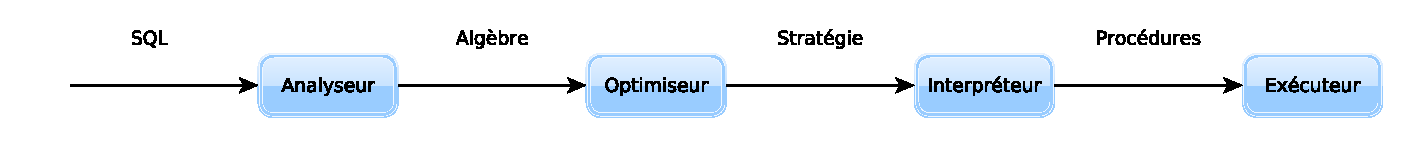
\includegraphics[width=0.9\textwidth]{rw-sgfd-optimsgbd}
\caption{Processus de traitement de requête dans un SGBD-R}\label{fig:rw:sgfd:optim:processus}
\end{figure}
Le seul composant ayant vraiment de l'intelligence est l'optimiseur. L'analyseur et l'interpréteur utilisent des routines déterministes et très strictes n'ayant qu'une seule sortie valable. L'optimiseur pourrait dans l'absolu sortir une stratégie égale au plan d'entrée avec les implémentations des opérateurs les plus simples (boucles imbriqués pour les jointures). Le résultat serait valable mais il est connu que le gain de l'optimiseur à l'exécution peut être immense\footnote{Des jointures bien placées sur les bons index peuvent transformer plus de 24 heures en moins d'une seconde}. 

Le problème est que l'espace des stratégies possibles pour exécuter une requête classique est potentiellement de cardinalité factorielle en fonction du nombre d'opérateurs et de méthodes d'exécutions disponibles (surtout s'il y a des jointures). Ainsi il faut guider l'exploration et utiliser des techniques de programmation dynamique pour éliminer rapidement les branches trop coûteuses.

\subsubsection{L'exploration de l'espace algébrique}
L'espace algébrique est le plus large car les équivalences de Codd~\cite{Codd:model} sont très larges et permissives. Ainsi même pour un arbre de requêtes avec moins d'une dixaine d'opérateurs cela peut monter à plus d'un millions de requêtes équivalentes si on peut permuter les opérateurs entre eux (très courant en algèbre de Codd). On sait de plus, que l'on peut rajouter des opérateurs sans que cela n'altère le résultat, l'exemple classique étant la projection.

Ainsi, on peut émettre plusieurs règles désormais connues pour éliminer un grand nombre d'arbres sous-optimaux :
\begin{itemize}
    \item[\textbf{R1}~:] La sélection et la projection n'introduisent pas de coût supplémentaires et sont traités à la volée. Les sélections doivent être exécutés au moment de la première lecture sur la relation. Les projections doivent se faire en même temps que le résultat d'un autre opérateur.
    \item[\textbf{R2}~:] Les produits cartésiens ne doivent jamais être formés sauf si la requête elle-même en demande. Seuls les jointures peuvent combiner des relations.
    \item[\textbf{R3}~:] L'opérande interne (partie droite) de chaque jointure est une relation originelle, et non un résultat intermédiaire
\end{itemize}

La règle R1 est certes discutable dans le cadre requêtes sans jointure (bien qu'elle fournisse dans ce cas des requêtes tout à fait valables). Toutefois, dans le cadre des requêtes plus complexes, elle permet de fixer une fois pour toute les opérateurs de sélection et projection. Cela restreint énormément le nombre de possibilités car dans toutes requêtes il y a une majorité de ces opérateurs (d'où l'utilité de les fusionner avec d'autres). Cela ne supprimera pas l'optimal car si on considère à juste titre le surcoût nul, les sélections seront proches des indexes et les projections seront minimales car on n'hésite pas à en introduire.

La règle R2 supprime toute possibilité de recours fatal aux algorithmes de boucles imbriqués alors qu'un autre plan pouvait utiliser à chaque fois des jointures plus efficaces.

La règle R3 n'est pas toujours implémentée car même si elle réduit beaucoup les possibilités car elle restreint les ordres de jointures, elle risque de supprimer l'arbre optimal dans plusieurs cas. En effet, les arbres de requêtes ne pourront pas être des arbres équilibrés car l'opérande droite doit être une relation native, or un arbre déséquilibré peut introduire des surcoûts du fait que les jointures supérieur doivent joindre une grande table avec un résultat intermédiaire. Toutefois, il existe des raisons à cette règle. Tout d'abord, le fait d'avoir des relations natives permet l'utilisation d'index. De plus elle permet de faire un traitement total des requêtes en mode pipeline\footnote{L'exécution en pipeline permet de traiter un tuple dès sa lecture, cela s'apparente à du traitement de flux. L'avantage est que le CPU étant moins coûteux que les I/O, on peut rentabiliser l'attente de lecture en traitement de requête.}.

En parcourant l'espace algébrique des requêtes équivalentes vérifiant R1-3, on trouve un nombre raisonnablement faible de plans pour savoir quelle sera la meilleur stratégie. 

\subsubsection{Le planning}
Le planning correspond au parcours de l'espace des méthodes disponibles pour chaque plan de requête et à l'évaluation de chacune de celles-ci. L'espace des méthodes fournit plusieurs implémentation pour un opérateur. Principalement dans les bases de données, on est en présence de trois jointures différentes : 
\begin{itemize}
    \item \textbf{Boucles imbriqués} : Implémentation la plus directe de la jointure. Cet algorithme ne requiert aucune condition sur les relations d'entrées. Il est malheureusement très lent dans la plupart des cas.
    \item \textbf{Jointure fusion} : Se base sur le fait que les deux relations sont triés sur l'attribut de jointure à l'avance. Ainsi la jointure est plus facile à effectuer. Elle est régulièrement utilisée avec des index triés comme les arbres B+. Des opérateurs de tri pourront être déployés. 
    \item \textbf{Jointure hachée} : Se base sur le fait que les deux relations sont hachées sur l'attribut de jointure. Ainsi la jointure se fait sur les index de hachages de cardinalité réduite et d'accès rapide. 
\end{itemize}

Or pour chaque relation, on peut accéder aux tuples vérifiant une sélection de deux façons différentes : 
\begin{itemize}
 \item \textbf{Scan} : On parcourt la relation ou l'index pour trouver les n-uplets vérifiant la sélection.
 \item \textbf{Probe} : On demande directement aux procédures d'index de renvoyer les tuples vérifiant la sélection. 
\end{itemize}

Ainsi, il est possible de faire des boucles imbriqués suffisamment performantes en utilisant des accès optimisés aux relations. Bien évidemment certaines sélections sont impossibles via les procédures d'index. Par exemple, il est impossible de demander à un index haché de faire une sélection avec un opérateur de comparaison tel que <<$\leq$>>.

L'évaluation de chacune de ces méthodes passe par un coût global de l'exécution que l'on base sur des statistiques de chacune des relations. Ces statistiques peuvent changer radicalement l'évaluation même en présence d'index. Supposons que l'on ai deux relations, l'une est hachée sur un attribut intéressant et l'autre est équipée d'un arbre B+ sur le même attribut. On souhaite désormais faire une jointure naturelle entre ces relations. Le plan qui sera sûrement utilisé si la première possède un cardinal similaire par rapport à l'autre, sera la jointure par fusion car le coût de tri sera négligeable. Ainsi on pourra faire une jointure extrèmement rapide en faisant la fusion directement sur l'accès à l'index. Dans le cas où le cardinal est négligeable, il sera préférable de faire un parcours direct en utilisant l'accès en $\mathcal O(\log N)$ de l'arbre B+. 

La recherche dans cet espace de méthode se base sur la programmation dynamique. Elle permet de faire une recherche exhaustive sans être extrèmement coûteuse. On ne détaillera pas l'algorithme ici mais le principe reste basé sur un \textit{branch \& bound} classique.

\subsubsection{Calcul de sélectivité}
Lorsque l'on fait une optimisation, on a vu que les statistiques étaient nécessaires. Cependant, si l'on veut calculer la taille des résultats intermédiaires, il est nécessaire de calculer les facteurs de sélectivité. 

On peut tout d'abord assumer l'uniforme répartition des données et appliquer y appliquer une sélectivité en fonction des différents cardinaux~\cite{Selinger:selectivity} (de l'index notamment\footnote{Un cardinal d'index est le nombre de valeur différentes que peut prendre un attribut, les doublons ne sont pas comptés.}), on remarque que l'on prend $\frac{1}{10}$ par défaut s'il nous manque des informations. Cependant, l'uniformité est rarement présente dans la pratique et ce genre d'assomption est erroné.

On se base généralement sur les résultats d'un ensemble de statistiques. La plupart utilisent le principe des histogrammes. Ceux-ci forment des ensembles de classes d'équivalence (buckets), classiquement de cardinaux (d'index) similaires, et à chaque classe on calcule au fur et à mesure sa fréquence d'apparition. Pour des raisons de simplicité, les classes sont formés suivant l'ordre naturel.

D'autres propositions ont été faites dans le milieu de la recherche mais seule la méthode des histogrammes à pas constant reste utilisée.

\subsubsection{Autres principes d'optimisation}
\paragraph*{Optimisation de la recherche}
La recherche exhaustive peut être très coûteuse si les jointures sont nombreuses car l'espace des stratégies devient immense. Bien heureusement, la plupart des requêtes usuelles se limite en dessous de la dixaine. Toutefois, en cas de grand nombre, une approche heuristique est nécessaire pour avoir un temps de calcul qui permette un lancement rapide de la requête. 

Plusieurs approches existent, la plus connue reste basée sur la marche aléatoire sur le graphe des stratégies possibles. Celle-ci parcourt le graphe aléatoirement en reculant si le coût est devenu trop important. Une autre approche intéressante étant l'utilisation d'algorithmes génétiques pour résoudre ce problème. Postgres utilise leur optimiseur \textit{Genetic Query Optimizer (GEQO)}~\cite{Postgres:geqo} si le nombre de jointure dépasse une certaine limite.

L'optimisation a été prouvée comme un problème NP-complet~\cite{Ibaraki:join} (même avec seulement les boucles imbriqués) ainsi certains efforts se sont concentré sur la résolution de sous cas importants, notamment boucles imbriqués et jointure hachée seulement.

\paragraph*{Base de données parallèles}
L'optimisation en prenant en compte des modèles de calculs parallèles est un problème encore ouvert. Toutefois. de bonnes approximations se basent sur les optimisations à deux phases. Tout d'abord, on cherche la solution optimal comme vu précédemment. Par la suite, on cherche le meilleur ordonnancement. Les deux domaines ont étés suffisamment couvert pour obtenir des résultats satisfaisants.

\paragraph*{Distribution du calcul}
La distribution du calcul est un problème différent des bases parallèles dans le sens où il existe plusieurs unités d'évaluation complètement indépendantes. Le problème toutefois se résout simplement en considérant la distribution du calcul à l'intérieur de l'espace des méthodes. L'espace de recherche sera toutefois plus grand et il faudra faire attention à avoir un optimiseur performant pour ne pas avoir de surcoût avant l'exécution.

\paragraph*{L'optimisation sémantique}
En supposant que l'on ai une base de connaissance en parrallèle de notre base de donnée. Il est alors possible de raisonner sur les conditions de sélections notamment, afin d'amener plus ou moins de restriction à la requête. Les calculs de subsomptions de concepts permettent d'avoir des résultats déjà pertinents à la sortie des sources ou des index. Le problème étant d'avoir une base de connaissance suffisamment exploitable et absolument à jour car une erreur de raisonnement pourrait supprimer potentiellement des résultats.

\subsection{Traitement de requêtes}
\subsubsection{Jointures}
Comme on le sait~\cite{Petit:astral}, la jointure en flux n'est pas aussi simple qu'une jointure au sens base de données. Beaucoup de travaux~\cite{Han:join, Srivastava:join, Law:join} se sont portés sur les jointures similaires à $I_S (S_1[\alpha_1,\beta_1,r_1] \Join ... \Join S_n[\alpha_n,\beta_n,r_n])$ et bien souvent avec des fenêtres identiques. Car l'implementation de ceci requiert a priori une quantité non bornée de mémoire. De plus le traitement d'un n-uplet prendra du temps et il faudra pouvoir fournir le résultat sans retard par rapport aux flux d'entrées. 

Afin de garantir une exécution en temps réel, des procédés de load-shedding~\cite{Tatbul:load-shedding} sont mis en place en essayant de maximiser la pertinence des résultats. On sort donc du contexte de l'exécution exacte de requête. Le principe de base réside dans le fait de garder les n-uplets étant les plus pertinent. Ceci peut être basé sur le nombre de n-uplet que le n-uplet produira après calcul, ou celui qui est le plus agé. Le calcul de ceci peut se faire de façon différente :
\begin{itemize}
 \item Par un histogramme et un choix sur le nombre de tuple résultant~\cite{Han:join}
 \item Par un calcul probabiliste pour privilégier un flux plutôt qu'un autre pour sa productivité~\cite{Han:join}
 \item Par des raisonnements sur l'age du n-uplet~\cite{Srivastava:join}
\end{itemize}

Toutefois, le traitement des jointures peut se faire de façon exacte et optimisés. Tout d'abord, il est notable de voir que des procédés d'indexations serait tout à fait utile. En effet, supposons que l'on puisse transmettre ou construire un index d'une relation. Ainsi, il sera possible de faire des jointures aussi optimisés que dans les bases de données. L'espace des méthodes est aussi conservé, toutefois le coût de telles solutions reste à évaluer car comme on le sait, les données changent fréquemment. Il devient donc difficile de maintenir les index. Les optimisations présentes dans le calcul de jointures relationnel en \textit{pipeline} sont ici bien évidemment applicables telles que le \textit{symmetric hash join}~\cite{Wilschut:symetricjoin}. 

D'autres optimisations ont étés abordés sur la distribution du calcul~\cite{Zhou:pmjoin}. En effet, le coût engendré par les échanges fait que le calcul de la distribution des opérateurs devient importante. Dans cette optimisation, il est important de prendre en compte le partitionnement de la charge du flux par rapport au domaine des attributs de jointures. En effet, un attribut pourra avoir un débit très faible sur une valeur comparé à un autre qui sera bien plus présent. Des optimisations sur la distribution de ces calculs sont faisable.

Enfin, de façon un peu plus particulière, il est intéressant de noter les optimisations dans des contextes particuliers tels que le P2P (avec une DHT)~\cite{Palma:p2p}. Le calcul de la jointure peut se faire sur plusieurs noeuds afin de mieux distribuer le traitement.

\subsubsection{Fenêtrage et agrégations}
Les problèmes de fenêtrage sont très similaires aux problèmes de jointures (qui nécessitent une fenêtre). Ici, on s'intéresse plus particulièrement aux calculs d'agrégation $I_S(G(S[\alpha,\beta,r]))$. Les travaux les plus conséquents se focalisent sur le fait de calculer des opérations de comptage et de quantile en mémoire limité~\cite{Arasu:window}. On remarque qu'avec ce genre de données les autres statistiques sont faisable en quantité restreinte~\cite{Datar:stats}, on note pouvoir faire (toujours de façon approximative) : 
\begin{itemize}
 \item Min/Max/Sum/Avg 
 \item Moyennes
 \item Tables de hachages
 \item Histogrammes
 \item Nombre de valeurs distinctes
\end{itemize}

L'approche est principalement mathématique et probabiliste et je ne rentrerai pas dans le détail. Il faut juste savoir qu'en se fixant une tolérance $\varepsilon$, on peut obtenir un résultat dans une quantité de mémoire qui peut être prévisible.

Cet ensemble de calculs pourra servir pour faire une base de statistiques en vue d'évaluations futures.
\subsubsection{Désignation}
La désignation est une opération coûteuse car elle nécessite de parcourir a priori l'ensemble du réseau pour savoir si telle ou telle source vérifie les conditions que l'on a posé. Des structures d'index ont étés ainsi mises en place notamment dans les réseaux de capteurs~\cite{Greenstein:difs}. Principalement, le but reste de pouvoir faire des recherches de device sur des données de haut niveau sémantique. Par exemple, il peut être utile de savoir qu'un groupe de capteur possède une température entre 20 et 30ºC. Ce qui fait que lors de la recherche d'un capteur émettant entre 20 et 25ºC, il suffira d'affiner la recherche dans ce groupe ci. 

Des recherches probabilistes se sont penchés dessus~\cite{Bhattacharya:mist}, en permettant de prédire le comportement d'une donnée au fur et à mesure du temps avec des chaines de Markov. Cette structure de données fournit un très bon contexte de désignation <<rapide>>.

Bien évidemment, toutes les recherches sur les infrastructures distribués permettent de répondre en terme d'optimisation. Par exemple, que ce soit des infrastructures de gestion de données de devices directement~\cite{Gurgen:sstreamware}, ou tout simplement dans le contexte P2P, l'utilisation de DHT.
\subsubsection{Historique}
Le stockage historique est une partie peu abordée dans le monde des flux de données car celle-ci passe directement dans le monde des bases de données qui sont connues maintenant. Toutefois le contexte des flux de données fait que d'autres optimisations peuvent être opérées. Un des travaux fondateurs serait~\cite{Chandrasekaran:oscar} qui avance le fait que les structures d'index habituelles (arbres B+) ne sont pas optimales dans ce contexte. En effet, l'index portant sur le \textit{timestamp}, et l'insertion se faisant presque toujours dans l'ordre croissant il est facile de trouver une structure plus adaptée. Comme beaucoup de travaux, celui-ci apporte le fait de pouvoir s'adapter à la charge en supprimant certains n-uplets à l'avance.

Pour ne pas perdre de données, il faut ainsi se tourner vers le domaine des \textit{data-warehouses}~\cite{Chaudhuri:warehouse} afin d'avoir de bonnes performances à l'insertion. Seulement, leur modèle de donnée fait que les requêtes auront du mal à être optimisés pour un résultat rapide. Des approches plus consensuelle~\cite{Petit:historical} ont étés mises en place pour s'adapter à la charge (en jouant sur le retard à l'insertion) sans perdre de données. Bien sûr, on introduit ainsi une limite de traitement. 

Enfin, un dernier mode de stockage sont les informations résumés~\cite{Diao:stonedb}. En effet, en considérant que l'on stocke à l'intérieur de la base de données des moyennes ou des images en moindre résolutions (pour les caméras), on peut gagner énormément en performances sans grandement détruire la sémantique du stockage. Certains travaux~\cite{Diao:stonedb} proposent de stocker au plus proche des appareils les données détaillés et d'utiliser les passerelles réseaux comme cache avec des données résumés. Les résumés peuvent être issus de la communauté du data mining. 
\subsection{Problèmes spécifiques}
\subsubsection{Load-shedding}
Comme vu précédemment, le but de l'optimisation n'est pas toujours de pouvoir fournir les résultats exacts aux requêtes. L'objectif étant de fournir les résultats les plus pertinents possibles avec des contraintes d'espace mémoire, de temps de réponse ainsi que de charge réseau. Plusieurs propositions ont déjà étés abordés pour des opérateurs  spécifiques présentés ci-dessus. 

On remarquera tout de même que la communauté scientifique s'est rapidement tournée vers cette étude. Car au delà de sa complexité théorique, le calcul de requêtes continues fait que l'on ne peut se permettre d'introduire un retard. Lors d'une requête ponctuelle, le traitement de celle-ci peut durer plusieurs minutes dans certains cas mais cela ne va pas entrainer de problème au delà de la charge inhérante au serveur. Dans le cadre des requêtes continues, si le débit de n-uplet à l'entrée est trop fort comparé au nombre maximal que l'arbre de requête peut traiter, alors on introduira un retard qui se cumulera au fur et à mesure, ce qui n'est pas gérable.

L'idée du load-shedding est de pouvoir abaisser le taux de n-uplet au nombre suffisant pour pouvoir traiter sans introduire de retard. L'optimisation des opérateurs implique des connaissances très particulières sur chacun de celui-ci (statistiques etc...). Le load-shedding global existe aussi. Dans les travaux fondateurs~\cite{Tatbul:window,Tatbul:load-shedding}, l'idée est de pouvoir surveiller le traitement des requêtes afin de reconnaitre les points d'engorgements et d'y implanter des opérateurs de shedding. Afin de garantir un certain taux de réussite, la politique qui sera utilisée pour le load-shedding sera dirigée par un \textit{QoS}\footnote{QoS : Quality of Service} déterminant quelles données sont utiles. En effet, en prennant en entrée un graphe représentant \textit{valeur} $\mapsto$  \textit{taux de suppression acceptable}. Par exemple, dans le cadre d'une surveillance d'incendie, le taux de shedding pour les températures inférieure à 20ºC pourra être très fort de part et d'autre du systèmes pour ce genre de données.

\subsubsection{Multi-Query Optimization (MQO)}
Aussi connu sous le nom de \textit{Global Query Optimization}. Cette optimisation profite des exécutions parrallèles pour éviter la redondances de traitement et une économie de ressources. Elle est issue du monde des base de données~\cite{Sellis:mqo} et permet de répondre à plusieurs requêtes en même temps en utilisant des parties communes (classiquement, lorsque seules les clauses de sélection sont différentes). L'idée est toutefois peu exploitée car il faut pouvoir soumettre plusieurs requêtes en même temps et les caches ont permis de faire de bon résultat pour ce genre de requêtes. 

Dans le monde des flux de données, cette optimisation est largement reconnue comme importante. Les requêtes durant dans le temps, de façon potentiellement infinie, le nombre d'exécution concurrente sera donc très grand. Ainsi, partager les ressources des requêtes devient une façon d'optimiser grandement les requêtes. Plusieurs points interviennent ici.
\begin{itemize}
 \item Tout d'abord l'existence des \textit{m-op} (multi-operators)~\cite{Hong:mqo}. Ces opérateurs permettent de regrouper plusieurs opérateurs en un seul permettant d'éviter des duplicatas de n-uplets. Un exemple classique étant de grouper deux sélections sur un flux commun en une seule. Ainsi, si un n-uplet vérifie les deux sélections, un seul n-uplet sera fournit avec l'indication qu'il appartient aux requêtes 1 et 2. Cette optimisation permet de faire des requêtes en utilisant les définitions de flux fragmentés.
 \item La synchronisation des sous-requêtes. Les requêtes ont a priori peu de chance d'être démarrées en même temps. Or il a été démontré que le temps de démarrage des requêtes est très important et fixe la sémantique de certains opérateurs. Ainsi deux sous-requêtes, même si leurs expressions sont identiques, ne sont pas garanties d'être partageables. C'est un problème peu abordé, souvent évoqué dans les travaux futurs. Des propriétés d'Astral permettent d'établir l'équivalence à travers le temps des requêtes. 
 \item Grande disponibilité des ressources. Chaque opérateur utilise des ressources et peut potentiellement les partager avec d'autres. Cependant, ces ressources ne sont peut-être pas utiles à partager car elles sont trop précises. Dans plusieurs travaux~\cite{Arasu:resource}, le calcul des agrégations sur fenêtres peut être partagé. En découpant la mémoire par bloc de façon intelligente, on peut partager les ressources afin d'économiser de la place mémoire.
\end{itemize}

Un problème ouvert reste de savoir si les optimisations locales (optimisation algébrique) gêneront les optimisations globales. C'est ainsi que l'on remarque qu'une requête ne possède pas qu'une seule optimisation au début de son traitement. En effet, si une nouvelle requête arrive et qu'en changeant légèrement la structure de la première, on peut obtenir un partage, alors il est probable que ce plan soit le bon.

\subsubsection{Ordonnancement}
L'exécution d'une requête utilise une grande quantité de buffers. Hors les tailles de ceux-ci sont bornés. En cas de surcharge notamment, il est important de pouvoir controler le trafic et l'engorgement des opérateurs. On peut certes réguler via des procédés de shedding mais on peut aussi permettre de prioriser le traitement des opérateurs ayant une faible sélectivité. Plusieurs stratégies ont étés proposés~\cite{Babcock:chain, Jiang:scheduling} afin de garantir le meilleur taux de réponse ou le moins de resources nécessaires.

\subsubsection{Routage}
Le problème du routage est un problème très connu des chercheurs du domaine des réseaux de capteurs où les contraintes de traitement sont si fortes au niveau de la transmission de données que les routages sont importants. Pour le traitement middleware de grandes quantités de données, des optimisations de routages rentrent en compte sur le calcul de jointure par exemple~\cite{Zhou:pmjoin}. En effet, il nous faut savoir s'il vaut mieux effectuer une opération lourde et ayant une sélectivité peut-être grande (>1) de façon distribuée avec transfert réseaux ou groupés mais plus chargés en CPU. 

D'un autre coté, le coût (énergétique ou autre) est analysé afin de fournir un routage au moment du placement de la requête~\cite{Galpin:snee} ou à l'exécution~\cite{Madden:tinydb}.

\subsection{Espace algébrique}
Malheureusement, cette section ne sera pas bien remplie. L'équivalence algébrique sur les opérateurs de flux de données et une chose très peu abordée. Plusieurs travaux mettent en avant le respect des équivalences initiales de l'algèbre relationnelle. Un des résultat les plus utilisé étant la poussée des projections. C'est un résultat efficace, très simple (car la permutation avec la projection est autorisé sur tous les opérateurs) donc souvent appliqué. 

L'utilisation de sélection au plus proche des sources est aussi un excellent moyen d'optimisation. Seulement, il a été prouvé que $\sigma_c R_S^u \neq R_S^u \sigma_c$ et que $\sigma_c S[D] \neq (\sigma_c S)[D]$ dans des cas où les bornes de $D$ sont positionnelles\footnote{Toutefois, $\sigma_c S[D] = \sigma_c (\sigma_c S)[D]$ dans tous les cas}. On ne peut donc pas a priori pousser les sélections au plus bas sans prudence au préalable, ce qui rend les possibilités bien limitées car ce sont des opérateurs courants.

Les recherches sur les meilleures configurations de jointures sont plus rares, car il faudrait disposer de statistiques précises pour établir un plan correct. De plus, un des principes qui permettait une vrai recherche n'est plus actif : la disymétrie de tout opérateur de jointure sur flux. 
